
%%% Local Variables:
%%% mode: latex
%%% TeX-master: t
%%% End:

\section{再认识与展望}

\begin{frame}[t]{加大现有数据的利用率}
\begin{itemize}
\item<1-> 面向业务的数据整合
\item<2-> 查询功能设计与开发
\end{itemize}

\begin{overlayarea}{\textwidth}{\textheight}
  \begin{onlyenv}<1>
\begin{figure}
  \centering
  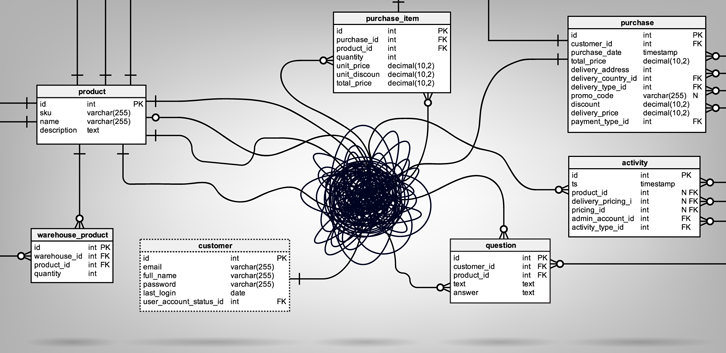
\includegraphics[width=\textwidth]{chp05_传统调查数据整合.png}
  \caption{数据整合要梳理数据结构特征,设计面向业务的数据库对象}
\end{figure}
  \end{onlyenv}

\vspace{-15pt}
  \begin{onlyenv}<2>
\begin{figure}
  \centering
  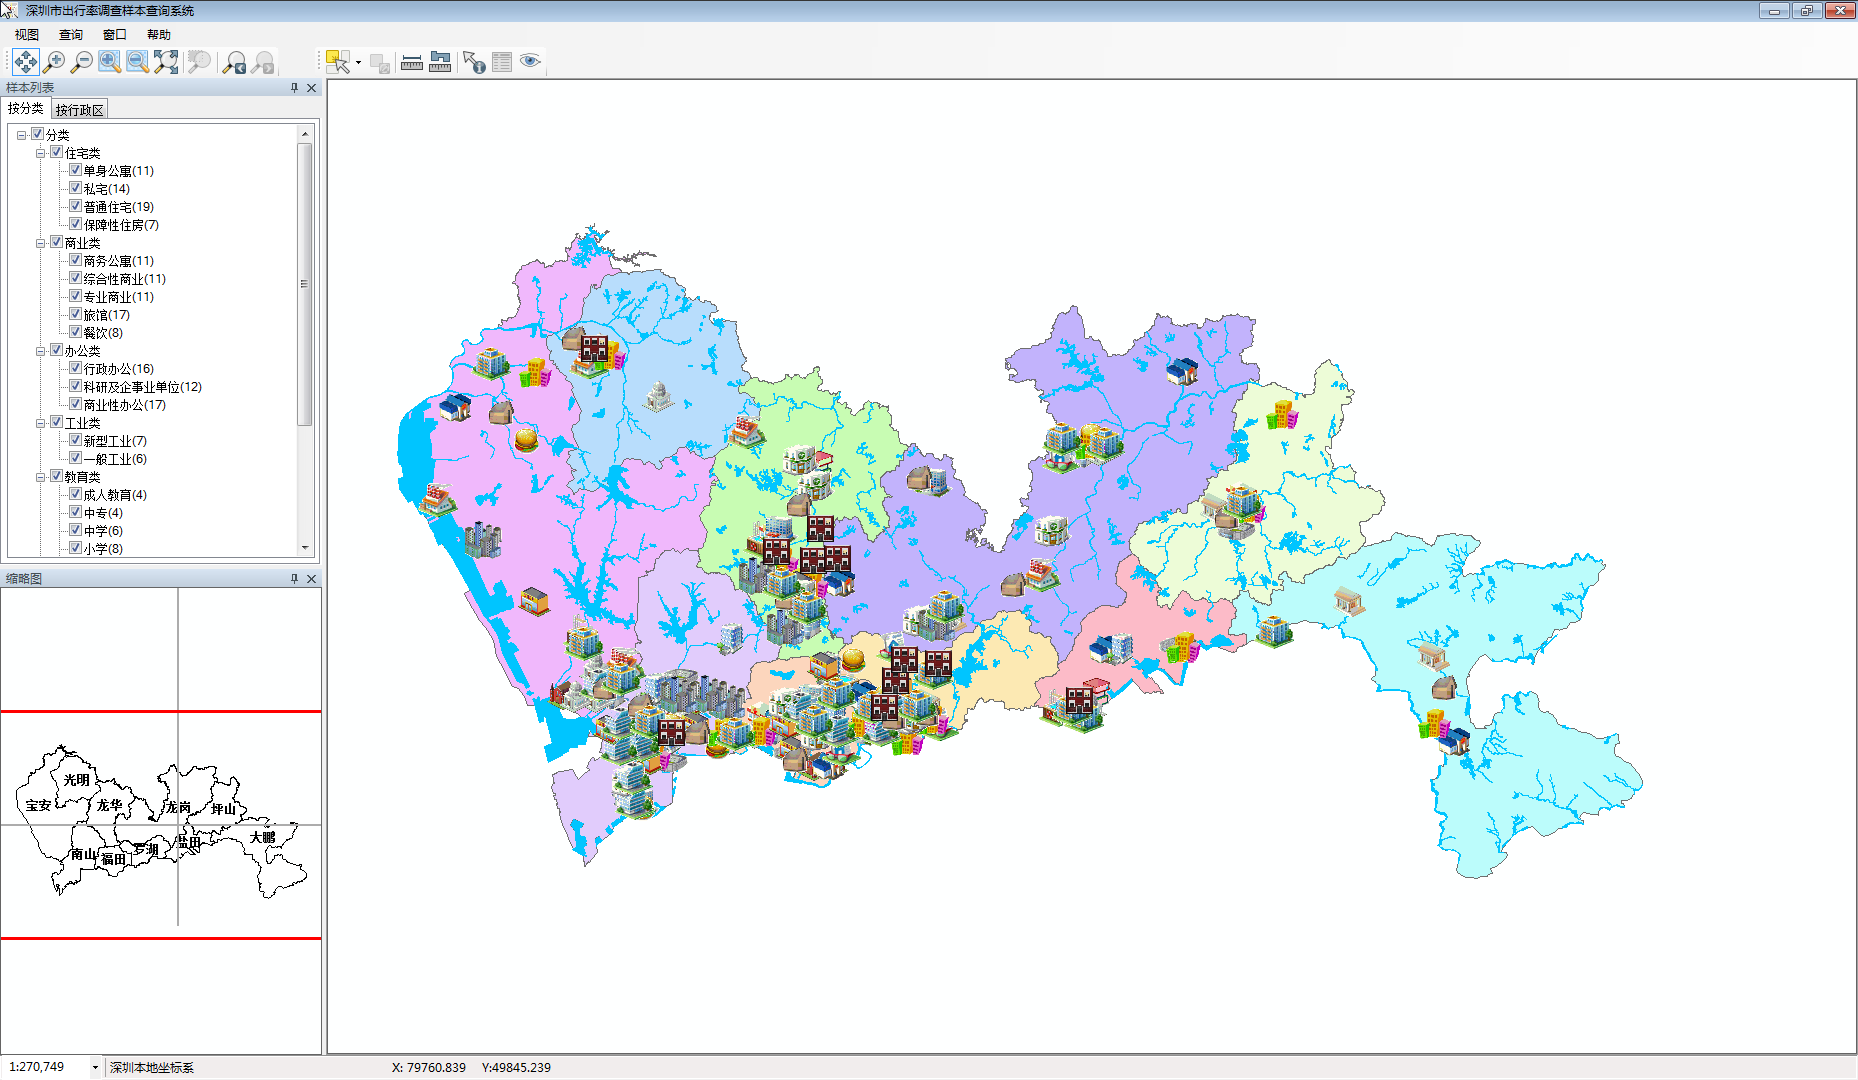
\includegraphics[width=\textwidth]{chp05_数据查询系统.png}
  \caption{基于GIS开发面向业务人员的数据查询系统}
\end{figure}
  \end{onlyenv}
\end{overlayarea}
\end{frame}

\begin{frame}[t]{提升数据分析的深度}
\begin{itemize}
\item<1-> 现有数据应用主要在传统交通模型和现状的简单指标统计,没有形成分析方法体系,
和金融、互联网、商业咨询等数据利用率高的行业相比\emphText{分析程度非常低下}
\item<2-> 交通模型体系在大数据环境下的理论创新,以及空间分析、机器学习等技术手段在交通规划行业的广泛应用
\end{itemize}

\end{frame}

\begin{frame}[t]{与业务结合开展新的应用研究方向}
\item 交通规划业务人员需要提升自身的技术水平,才能够提出具有可行性的需求
\item 分析人员要充分介入业务,主导应用研究的开展
\end{frame}

\begin{frame}[t]{“自下而上”的规划决策}

\end{frame}

\begin{frame}[t]{国家智慧城市建设战略的基础}

\end{frame}


